\chapter{Run-Time Network Performance Monitoring and Management for Distributed CPS Applications}
\label{ch:runTime}

%%%%%%%%%%%%%%%%%%%%%%%%%%%%%%%%%%%%%%%%%%%%%%%%%%%%%%%%%%%%%%%%%%%%%%%%%%%%%%%%%%%
%%%%%%%%%%%%%%%%%%%%%%%%%%%%%%%%%%%%%%%%%%%%%%%%%%%%%%%%%%%%%%%%%%%%%%%%%%%%%%%%%%%
%%%%%%%%%%%%%%%%%%%%%%%%%%%%%%%%%%%%%%%%%%%%%%%%%%%%%%%%%%%%%%%%%%%%%%%%%%%%%%%%%%%
%%%%%%%%%%%%%%%%%%%%%%%%%%%%%%%%%%%%%%%%%%%%%%%%%%%%%%%%%%%%%%%%%%%%%%%%%%%%%%%%%%%
%%%%%%%%%%%%%%%%%%%%%%%%%%%%%%%%%%%%%%%%%%%%%%%%%%%%%%%%%%%%%%%%%%%%%%%%%%%%%%%%%%%
\section{Middleware-Integrated Measurement, Detection, and Enforcement}
\label{sec:middleware}

\subsection{Problem}
Many networking solutions, especially for large-scale systems, utilize
a communications middleware of some sort, which allows the lower layer
networking implementations to be abstracted into a uniform application
programming interface.  Furthermore, these middleware often support
higher-level communications, resource management, and reliability
configurations than the lower layers they are built on.  However,
these middlewares do not support the kind of time-varying resource
constraints and provisioning which we have modeled and analyzed.
Similarly, the lower layer resource allocation supports only static
resource allocations, such as static bandwidth allocation for
different flows traversing a network link.

As an example of such static resource allocation, consider two flows
produced on the same node for the same network interface.  These flows
produce data with a rate that varies with respect to time, and both
flows are high-priority flows.  Since both flows are high-priority,
they should be guaranteed the data rate they need for the link they
share, but the link cannot support the combination of the flows'
maximum data rates, even though their maximum data rates do not happen
simultaneously.

With such resource allocation, it is difficult to guarantee these flows
the capacities they require while ensuring that excessive data
produced by one of the flows does not negatively impact the other
flow.  

\subsection{Results}
To address this static resource allocation problem, we have integrated
our modeling semantics into middlewares to provide time-varying
network resource allocation and capacity sharing.

Our run-time research and development of measurement, detection, and
enforcement code for networked applications is built on the foundation
of component-based software engineering (CBSE).  The goal of CBSE is
to provide a reusable framework for the development of application
building-blocks, called \emph{components} so that developers can develop
and \emph{analyze} applications in a more robust and scalable manner.  In
CBSE, a \emph{component}, shown schematically in
Figure~\ref{fig:component}, is the smallest deployable part of an
application and is defined as a collection of timers, ports, and a
executor thread:

\begin{equation}
  C = \{\{T\},\{P\},H\}
\end{equation}

Where

\begin{itemize}
\item $\{T\}$ is the \emph{set} of all \emph{timers} within the component.  A
  timer provides a periodic event trigger to the component which
  triggers the callback associated with $T$, where a callback is a
  function defined and implemented by the developer.  
\item $\{P\}$ is the \emph{set} of all \emph{input/output ports} within the
  component.  An i/o port provides a mechanism for message passing and
  event triggering between components, and may take the form of
  asynchronous \emph{publish/subscribe} or synchronous \emph{client/server}
  interaction patterns.  Similarly to timers, each incoming event
  triggers the callback associated with $P$.
\item $H$ is the single thread which executes all event events for
  the component, in FIFO order, without preemption.  
\end{itemize}

\begin{figure}[ht!]
  \centering
  \includegraphics[width=0.85\textwidth]{../doc/src/images/results/ros_component.png}
  \caption{Schematic representation of a software component.}
  \label{fig:component}
\end{figure}

From this component definition, we can define an application as a
grouping of components and a mapping between the ports of components:

\begin{equation}
  A = \{\{C\},\{M\}\}
\end{equation}

Where

\begin{itemize}
\item $\{C\}$ is the \emph{set} of components in the application
\item $\{M\}$ is the \emph{set} of \emph{mappings} between ports of
  the components in $\{C\}$, for instance connecting a subscriber of
  $C_x$ to a publisher of $C_y$, $M_{x,y} : C_x\{P_S\}\mapsto
  C_y\{P_P\}$.
\end{itemize}

And finally, an application's components are grouped into processes
and distributed onto the nodes of a system through a deployment
defined as a collection of nodes, processes, and a mapping from the
nodes to the processes:

\begin{equation}
  D = \{\{N\},\{U\},\{M\}\}
\end{equation}

Where

\begin{itemize}
\item $\{N\}$ is the \emph{set} of hardware \emph{nodes} in the system
\item $\{U\}$ is the \emph{set} of \emph{processes} defining the deployment,
  where a process is a collection of components
  $U=\{C\}\subseteq A\{\{C\}\}$.
\item $\{M\}$ is the \emph{set} of \emph{mappings} between processes and nodes
  in the system, e.g. $M_{U_1,N_1} : U_1\mapsto N_1$.
\end{itemize}

Note here that though the components are single threaded internally,
the application containing these components may run them in parallel,
e.g. by grouping them into a process or distributing them among the
hardware nodes of the system.  An example application and deployment
onto a system of nodes is shown in Figure~\ref{fig:cbse}.  Note that
multiple applications (shades of blue in this figure) may be deployed
simultaneously onto the same system and may even interact with each
other.

\begin{figure}[ht!]
  \centering
  \includegraphics[width=0.85\textwidth]{../doc/src/images/results/cbse.png}
  \caption{Two example distributed CBSE applications deployed on a system with
    4 nodes.}
  \label{fig:cbse}
\end{figure}
   
To facilitate experimentation and testing of our analysis techniques,
we have developed network traffic production and consumption code
which produces or consumes traffic on a communications link according
to either a sender profile or receiver profile.  These profiles are
the same profiles used in the design-time analysis.  We integrated
this producer/consumer code into our component code-generators, which
generate component skeleton code and communications middleware glue
code based on our component model.  Both sender and receiver
automatically measure and record the network traffic for offline
analysis.

Since the sender middleware code is automatically measuring and
recording the output traffic from the application, we implemented
additional code which can optionally push-back to the application by
throwing and exception when the application is producing more data
than specified in its profile.  This push-back helps prevent a single
application from producing more data than the system was designed for
and flooding the network.  In the case that such a push-back occurs,
the application is notified and the data is not transmitted onto the
network.  Using this mechanism, a malicious or faulty application can
be prevented from flooding the network and degrading the service of
the network to other applications.

Similarly, since the receiver middleware code is automatically
measuring and recording the input traffic from each of its senders, we
implemented an additional communications channel which is used by the
sender and receiver middleware and allows out-of-band communication
which is invisible to the application.  This out-of-band channel
allows the sender to detect anomalies and inform the sender-side
middleware of such anomalies.  Further details about this capability
and uses are explained in Section~\ref{sec:ddos}.

The development of this producer/consumer/measurement code not only
helps with running experiments and data collection but also helps to
ensure model to system consistency.
  
\begin{figure}[ht!]
  \centering
  \includegraphics[width=0.85\textwidth]{../doc/src/images/results/app_layers.png}
  \caption{The structure of component-based applications and how their network
   traffic traverses the middleware and the OS stack.}
  \label{fig:sender}
\end{figure}

We have implemented profile-based traffic production/consumption and
traffic measurement into our code generators that we use with our
model-driven design software.  We developed this toolsuite to create
distributed component-based software which uses the Robot Operating
System (ROS)\cite{ros} as the communications middleware.  ROS provides
the capability for managing message passing, event triggering, and
timer triggering that we need for our software components.  For
publish/subscribe interactions between components, into the
publisher's generated code we add generic traffic producer code which
publishes traffic according to the sender profile.  Additionally,
these publish operations are configured to use a small wrapper
function which can measure the publish rate and can decide to throw a
\emph{profile exceeded} exception if the application attempts to send
too much data or if the receiver has pushed back to the sender
informing it to stop.  The sender-side middleware layer is shown in
Figure~\ref{fig:sender}.

This push back from the receiver occurs through the use of an
out-of-band (OOB) channel using UDP multicast, which receivers use to
inform specific senders that they are sending too much data to the
receivers (and possibly overflowing the receiver buffers).  This OOB
channel provides a mechanism by which the secure middleware layer can
protect the system from malicious or faulty applications.

Into the receiver code (for subscribers) we additionally generate a
receive buffer and receiver thread which pulls data from the buffer
according to the receiver profile.  In this scenario, the receiver has
a capacity with which it can handle incoming data, and it has a finite
buffer so it must use the OOB channel and measurements on the incoming
data stream to determine which senders to shut down to ensure its
buffer does not overflow.  When the buffer has had some time empty (so
that it's not in danger of running out of buffer space), the receiver
can use the OOB channel to inform the halted senders that it is
alright to send again.  The complete description of the OOB channel,
and the way the receiver limits the senders can be found in
Section~\ref{sec:ddos}.  An example of our traffic producer's accuracy
is shown in Figure~\ref{fig:generation}.  For the data in this figure,
each message was recorded as a tuple of $timestamp, message size$,
where the timestamp is the time at which the message was either sent
by the application.

\begin{figure}[ht!]
  %\centering
  \includegraphics[width=1.1\textwidth]{../doc/src/images/results/traffic_generation.png}
  \caption{Demonstration of the accuracy with which our traffic
    producers follow the specified profile.}
  \label{fig:generation}
\end{figure}

\iffalse

\begin{definition}[Note:]
The measured bandwidth profile is calculated based on
recorded time series data of $[reception\_time,
message\_size]$, so the bandwidth drops to nearly 0
periodically since the $\Delta t$ is so large between
the messages.
\end{definition}

\begin{definition}[Note:]
Our original implementation of traffic producers performed
	  better since they did not utilize a middleware layer and
	  relied instead on simple point to point ipv6 connections.
	  However, that code was less useful for system analysis
	  because it could do nothing aside from traffic production
	  and measurement; our current implementation which generates
	  traffic production code into component code is more
	  versatile for several reasons:

          \begin{itemize}
	  \item The component-based code integrates directly into our development
	    toolsuite and deployment framework so it can be easily deployed on
	    our cluster.
	  \item Configuring different system topologies or component to host
	    mappings (deployments) is simpler and more robust, allowing us to
	    perform more and more varied experiments.
	  \item The traffic production code can be removed (or the code can be
	    regenerated without the option selected) and the rest of the
	    component-based and middleware code is still useful as an actual
	    application.
          \end{itemize}
\end{definition}

\fi

\newpage
%%%%%%%%%%%%%%%%%%%%%%%%%%%%%%%%%%%%%%%%%%%%%%%%%%%%%%%%%%%%%%%%%%%%%%%%%%%%%%%%%%%
%%%%%%%%%%%%%%%%%%%%%%%%%%%%%%%%%%%%%%%%%%%%%%%%%%%%%%%%%%%%%%%%%%%%%%%%%%%%%%%%%%%
%%%%%%%%%%%%%%%%%%%%%%%%%%%%%%%%%%%%%%%%%%%%%%%%%%%%%%%%%%%%%%%%%%%%%%%%%%%%%%%%%%%
%%%%%%%%%%%%%%%%%%%%%%%%%%%%%%%%%%%%%%%%%%%%%%%%%%%%%%%%%%%%%%%%%%%%%%%%%%%%%%%%%%%
%%%%%%%%%%%%%%%%%%%%%%%%%%%%%%%%%%%%%%%%%%%%%%%%%%%%%%%%%%%%%%%%%%%%%%%%%%%%%%%%%%%
\section{Distributed Denial of Service (DDoS) Detection}
\label{sec:ddos}

\subsection{Problem}
For distributed systems which must ensure resource availability and
system stability, a key aspect of the infrastructure is detection and
mitigation of faults or anomalies.  With respect to network resources,
an example is checking source and destination for communications to
enforce only authorized communication flows are present in the system.
However, software glitches or compromised applications can exceed
system resources that they have been allocated.  As described in the
previous section, higher-fidelity resource modeling and monitoring is
required to prevent such faults or compromises from propagating
throughout the system.  However, mitigating the propagation only
solves part of the problem; ideally the system should classify the
type of fault or anomaly and begin diagnostics to trace the
fault/anomaly back to its origin.  In this thesis we will address only
the problem of detecting and mitigating Distributed Denial of Service
attacks.  

Denial-of-Service (DoS)\cite{rfc4732} and Distributed DoS (DDoS) attacks
can take many forms, but are generally classified as excessive traffic
from a large amount of (possibly heterogeneous) sources targeted
towards a single point or a single group.  Such attacks are common to
machines on the internet, but can also become a hazard for machines on
private networks which become infected or inadvertently expose an
input path for external malicious data.

These private or semi-private systems must have mechanisms for
detecting and mitigating such attacks, and the combination of our
design-time analysis and run-time measurement, detection, and
mitigation tools provides a form for such capability.  The goal of
this work is for a receiver, which is being targeted for attack by a
set of senders, to determine which of the senders are behaving
anomalously and prevent them from sending any more data.  In this way,
a group of senders performing a DDoS attack can be mitigated by the
targeted receiver.  Towards this goal we make the following changes
outlined below to our modeling/analysis framework and implementation.

\subsection{Results}
Because these types of attacks come from systems for which the
application profiles may not be completely or fully known, we must
alter our modeling semantics such that we can model these types of
applications and the uncertainty surrounding their data rates.  

If we relax the constraint on the modeling semantics that all
sender profiles are absolute and the system behavior is completely
known at design-time, then we not only expand the scope of
applications that can be supported but also enable meaningful anomaly
detection.

Whereas previously, profiles modeled the exact $data\ rate$ as a
function of time that the application produced, we now alter the
definition to capture two parameters: $mean\ data\ rate$ ($\mu$) and
$max\ data\ rate$ ($MDR$), which again are both functions of time.
Just as before, these functions are constant-valued between successive
values of $t$ and are time-integrated to produce the $mean\ data$ and
$max\ data$ cumulative profiles as functions of time.  With this
specification, we no longer know exactly how much data an application
will produce at a given point in time, but instead are provided two
values by the developer: the $mean$ and $max$.

Now that we have these two profiles for the application, we could
simply analyze the $max$ data profile to determine buffer and latency
requirements, but this would end up wasting resources by allocating
memory and network resources of the system to the application even if
is not producing data at its \emph{max rate}.  Instead, we analyze the
system according to the $mean$ data profile to determine buffer
requirements and latency for the application in the system.  In doing
so, two buffer overflow risks are possible: 1) Sender-side buffer
overflow, and 2) Receiver-side buffer overflow.

We make the assumption that the application meters its sending to
prevent the first scenario, so that its data is not lost before making
it onto the network.  In this case, the sender can still send data at
a rate greater than the $mean$, but that rate is partially
governed by the capacity given to it by the node's network.

For the second case, we must ensure that there is no buffer overflow
on the receiver-side.  To enable this functionality, we must provide a
mechanism for the receiver to communicate with the sender.  This
push-back communication should travel through a channel outside the
communications channel that the application has access to, so that the
application, either maliciously or inadvertently, cannot disrupt this
push-back and in turn cause the receiver's buffer to overflow.  For
this reason, we add into the sender and receiver middleware an
out-of-band (OOB) channel that provides a communications layer between
all senders and receivers that is invisible to the application.  For
our component model and communications middleware, we have implemented
this OOB channel as a UDP multicast group.

Because the goal of this work is to meter only the senders which are
producing \emph{too much} data, we must define what too much data is.
Because we have developed these application profiles for analysis, and
these profiles describe the mean data rate, $\mu$, and the max data
rate, $MDR$, of the senders, they will be used to determine when a
sender is sending too much data.  In this paradigm, sender $S_i$ is
determined as behaving anomalously (i.e. sending too much data) if it
is sending data at a rate $DR_i > \mu_i$.  The assumption implicit in
this comparison is that the receiver, to be able to make this
comparison, has full knowledge of $\mu_i$, since $DR_i$ is calculable
on the receiver side.  If the receiver's buffer is filling up, it
looks through the the measured $DR_i$ (within a certain window of
time) for each of the senders it has been receiving data from, and
compares it against the sender's $\mu_i$.  If the comparison is
\emph{true}, it uses the OOB channel to push back to that specific
sender, informing the sender-side middleware to stop transmitting data
until the receiver has re-enabled that sender's transmission.  When
the receiver has emptied it's buffer enough it can then use the OOB
channel to re-enable any disabled senders.  The algorithm used by the
receiver to determine which senders to limit is shown in
Listing~\ref{lst:ddos_alg}.

\begin{listing}[ht!]
  \begin{minted}{python}
  receiver::limit_ddos( t_start, t_end )
  {
    for sender in senders
    {
      d_start = sender.received_data(t_start)
      d_end = sender.received_data(t_end)
      profile_d_start =
        sender.profile(t_start)
      profile_d_end =
        sender.profile(t_end)
      allowed_data = profile_d_end - profile_d_start
      actual_data = d_end - d_start
      if actual_data > allowed_data
      {
        sender.disable()
      }
    }
  }
  \end{minted}
  \caption{Algorithm used by receivers to determine which senders to
    limit.  The receiver only looks at the behavior of senders within
    the time window between $t_{start}$ and $t_{end}$, which is
    configurable.}
  \label{lst:ddos_alg}
\end{listing}


\begin{figure}[ht!]
  \centering
  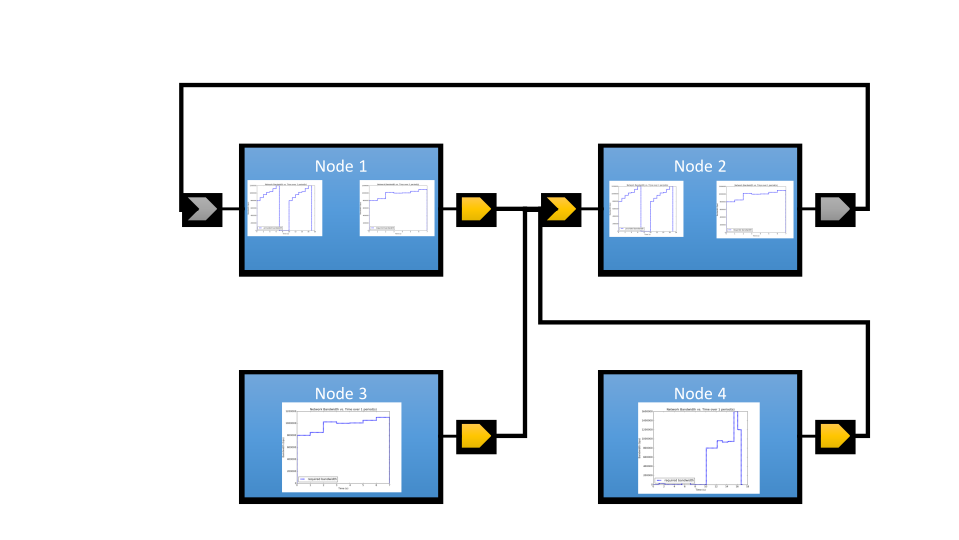
\includegraphics[width=0.85\textwidth]{../doc/src/images/results/example_setup.png}
  \caption{Nodes in an example network and how they communicate (using
    pub/sub).}
  \label{fig:ddos}
\end{figure}

We have implemented the OOB channel communication into our sender and
receiver component code along with the profile measurement and
comparison.  Using these code generators, we are able to run
experiments validating that the receiver can properly manage its
buffer by throttling excessive senders during times of congestion. 

We have shown experimentally (for the system in Figure~\ref{fig:ddos})
that, for example, a receiver side buffer size of 400000 bits, which
would normally grow to 459424 bits because of excessive data pumps on
the sender sides, is kept to 393792 by utilizing this out-of-band
channel and secure middleware.

\iffalse

%%%%%%%%%%%%%%%%%%%%%%%%%%%%%%%%%%%%%%%%%%%%%%%%%%%%%%%%%%%%%%%%%%%%%%%%%%%%%%%%%%%
%%%%%%%%%%%%%%%%%%%%%%%%%%%%%%%%%%%%%%%%%%%%%%%%%%%%%%%%%%%%%%%%%%%%%%%%%%%%%%%%%%%
%%%%%%%%%%%%%%%%%%%%%%%%%%%%%%%%%%%%%%%%%%%%%%%%%%%%%%%%%%%%%%%%%%%%%%%%%%%%%%%%%%%
%%%%%%%%%%%%%%%%%%%%%%%%%%%%%%%%%%%%%%%%%%%%%%%%%%%%%%%%%%%%%%%%%%%%%%%%%%%%%%%%%%%
%%%%%%%%%%%%%%%%%%%%%%%%%%%%%%%%%%%%%%%%%%%%%%%%%%%%%%%%%%%%%%%%%%%%%%%%%%%%%%%%%%%
\section{Network Resource Monitoring and Management Integrated into Component-Based Middleware}
\label{sec:drems}

\subsection{Problem}
Distributed, deployed CPS require design-time assurances of system
stability and security.  These assurances guarantee that resources and
communications must have some protection against propagating software
faults or malicious actors.  One such avenue for fault or attack
propagation is the system's communications network.  Systems provide
the computational resources, hardware access, and communications
required for their applications.  For example, the satellite cluster
provides (1) distributed processors which are shared by the
applications, (2) data from the on-board sensors provided by each
satellite, and (3) a wireless communications network.  During
deployment, the system enforces resource utilization limits on the
applications, e.g. memory or disk space limitations, which must be
broad to account for whatever the applications may need to do over
their lifetime.  However, application resource limits which do not
incorporate temporal behavior (i.e. static limits) are inefficient
since they waste resources allocated to applications not using them.
Furthermore, these static resource limits do not provide tight bounds
on application behavior and may create avenues for fault or attack
propagation.  An example of such resource reservation schemes
backfiring is a Distributed Denial of Service (DDoS) attack, in which
many compromised applications produce slightly more network traffic
than usual (but still within their limits) to produce a combined
network traffic profile that can effectively take their target off of
the network.

\subsection{Contributions}
\begin{itemize}
	\item We integrated our network resource modeling techniques
          into a system and application analysis and development
          tool-suite. The tool verified that the system could provide
          all the network resources (which varied as a function of
          time) required by the applications.  The accuracy of the
          predictions was described in
          Section~\ref{sec:experimentalVerification}.
	\item Into the application's generated middleware interface
          code we integrated measurement, detection, and mitigation
          code which (1) measured the characteristics of the
          application's network traffic, (2) detected if the
          application's network traffic exceeded its profile that was
          provided during system analysis, and (3) blocked all traffic
          from leaving application-space (i.e. it did not get into
          kernel-space) which was detected as having exceeded the
          profile.  We showed that this management code allowed
          properly shaped traffic onto the network and blocked
          improperly shaped traffic.
\end{itemize}

%%%%%%%%%%%%%%%%%%%%%%%%%%%%%%%%%%%%%%%%%%%%%%%%%%%%%%%%%%%%%%%%%%%%%%%%%%%%%%%%%%%
%%%%%%%%%%%%%%%%%%%%%%%%%%%%%%%%%%%%%%%%%%%%%%%%%%%%%%%%%%%%%%%%%%%%%%%%%%%%%%%%%%%
%%%%%%%%%%%%%%%%%%%%%%%%%%%%%%%%%%%%%%%%%%%%%%%%%%%%%%%%%%%%%%%%%%%%%%%%%%%%%%%%%%%
%%%%%%%%%%%%%%%%%%%%%%%%%%%%%%%%%%%%%%%%%%%%%%%%%%%%%%%%%%%%%%%%%%%%%%%%%%%%%%%%%%%
%%%%%%%%%%%%%%%%%%%%%%%%%%%%%%%%%%%%%%%%%%%%%%%%%%%%%%%%%%%%%%%%%%%%%%%%%%%%%%%%%%%
\section{Network Application Fault/Anomaly Classification}
\label{sec:classification}

\begin{itemize}
	\item We will use our testbed to run distributed network tests
          to classify certain types of anomalies, e.g. DDoS attacks
          from compromised applications within the cluster.
	\item We will use the network resource utilization
          measurements gained from the tests to derive metrics which
          allow us to differentiate between classes of behavior,
          e.g. standard/stable application behavior vs. DDoS behavior.
	\item We will then use the classifications to show that the
          system can detect these types of attacks, mitigate their
          propagation, and report the attack to the system's manager.
\end{itemize}

\fi
